\chapter{FLOCKING ALGORITHM}\label{chap3}

% introduction
%\section{Introduction}
The behavior seen in social animals like birds and fishes is called \textit{flocking}. Flocking can be used to simulate this social behavior between entities by following a set of simple rules. These rules were introduced by the pioneer of flocking Craig Reynolds\cite{craig1}. The three main steering behaviors are: separation, alignment, and cohesion. This chapter will discuss the different behaviors implemented in our code, which include the three main steering behaviors, along with a few others.

% 3 steering behaviors
\section{Three Main Steering Behaviors}
These steering behaviors are velocity vectors, they have direction and magnitude. Each behavior is evaluated at each time step for each boid.

% separation
\subsection{Separation}\label{separationsection}
\textit{Separation} can be described as the steering force that maintains each entity of the flock separated by at least a minimum determined distance. Craig Reynolds first called this rule \textit{collision avoidance} because he meant to avoid collision with nearby flockmates. Later on, the rule was named \textit{separation}. This steering behavior prevents crowding between boids. As can be seen in Figure~\ref{separationPDF} only flockmates within a certain radius when evaluating this behavior are considered. The red vector is the obtained steering force with this behavior.

% separation figure
\begin{figure}[htbp]
\begin{center}
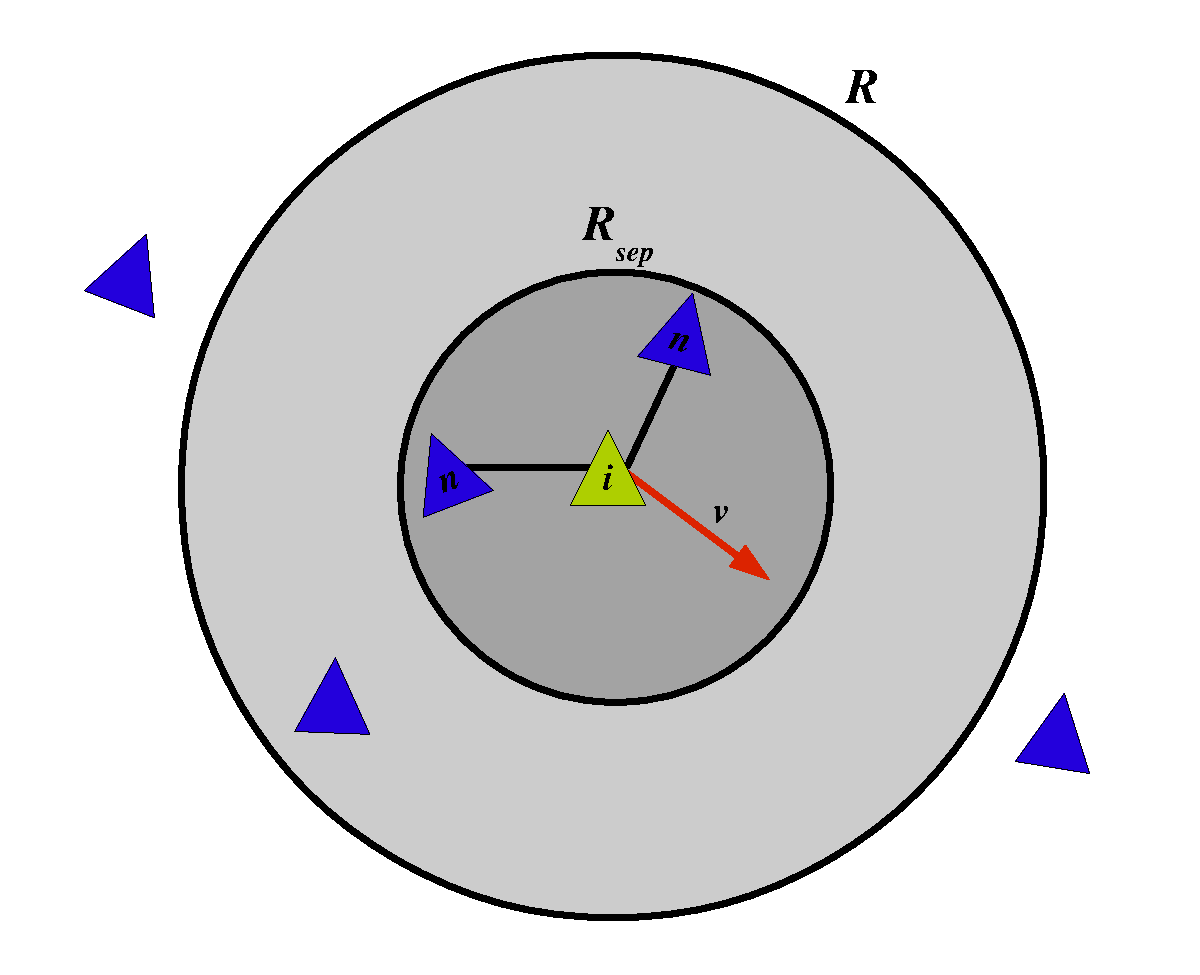
\includegraphics[scale=0.3]{figures/separation.pdf}
\caption{Separation steering force: the gray circle is the neighborhood of the green boid, \textit{separation} would steer the green boid away/near the neighboring boids until a minimum distance between them is met}
\label{separationPDF}
\end{center}
\end{figure}

Separation is a repulsive force. The mathematical expression that was implemented is showed in equation~\ref{separationEquation}.

% separation equation
\begin{equation}
\label{separationEquation}
Separation =\frac{1}{M} \sum_{n=1}^{M} \frac{p_i - p_n}{d(p_i,p_n)}
\end{equation}

Where $M$ is the number of boids within the minimum distance from the boid in question, $p_i$ is the position of boid $i$, and $d(p_i,p_n)$ is the distance between boids $i$ and boid $n$.

Looping over the nearest neighbors is the first step, then only neighbors that are with the minimum separation distance are picked. Next, is to sum up the difference between the positions of boid $i$ and boid $n$ divided by the distance of boid $i$ from boid $n$. Then, take the average over the number of boids that were within the minimum distance to finally get the the vector that is going to correct the heading and speed of the \textit{separation} of boid $i$  and their nearest neighbors. 

% alignment
\subsection{Alignment}
\textit{Alignment} is the steering behavior that match the heading of all boids. Reynolds initially called this behavior \textit{velocity matching}, later the name was changed to \textit{alignment}. This behavior also prevents crowding along with \textit{separation}. As the name of the rule said, each boid would \textit{align} itself with the average velocity of the local neighborhood. Align with respect of direction and/or speed. Figure~\ref{alignmentPDF}  shows the corrective steering force vector in red.

% alignment figure
\begin{figure}[htbp]
\begin{center}
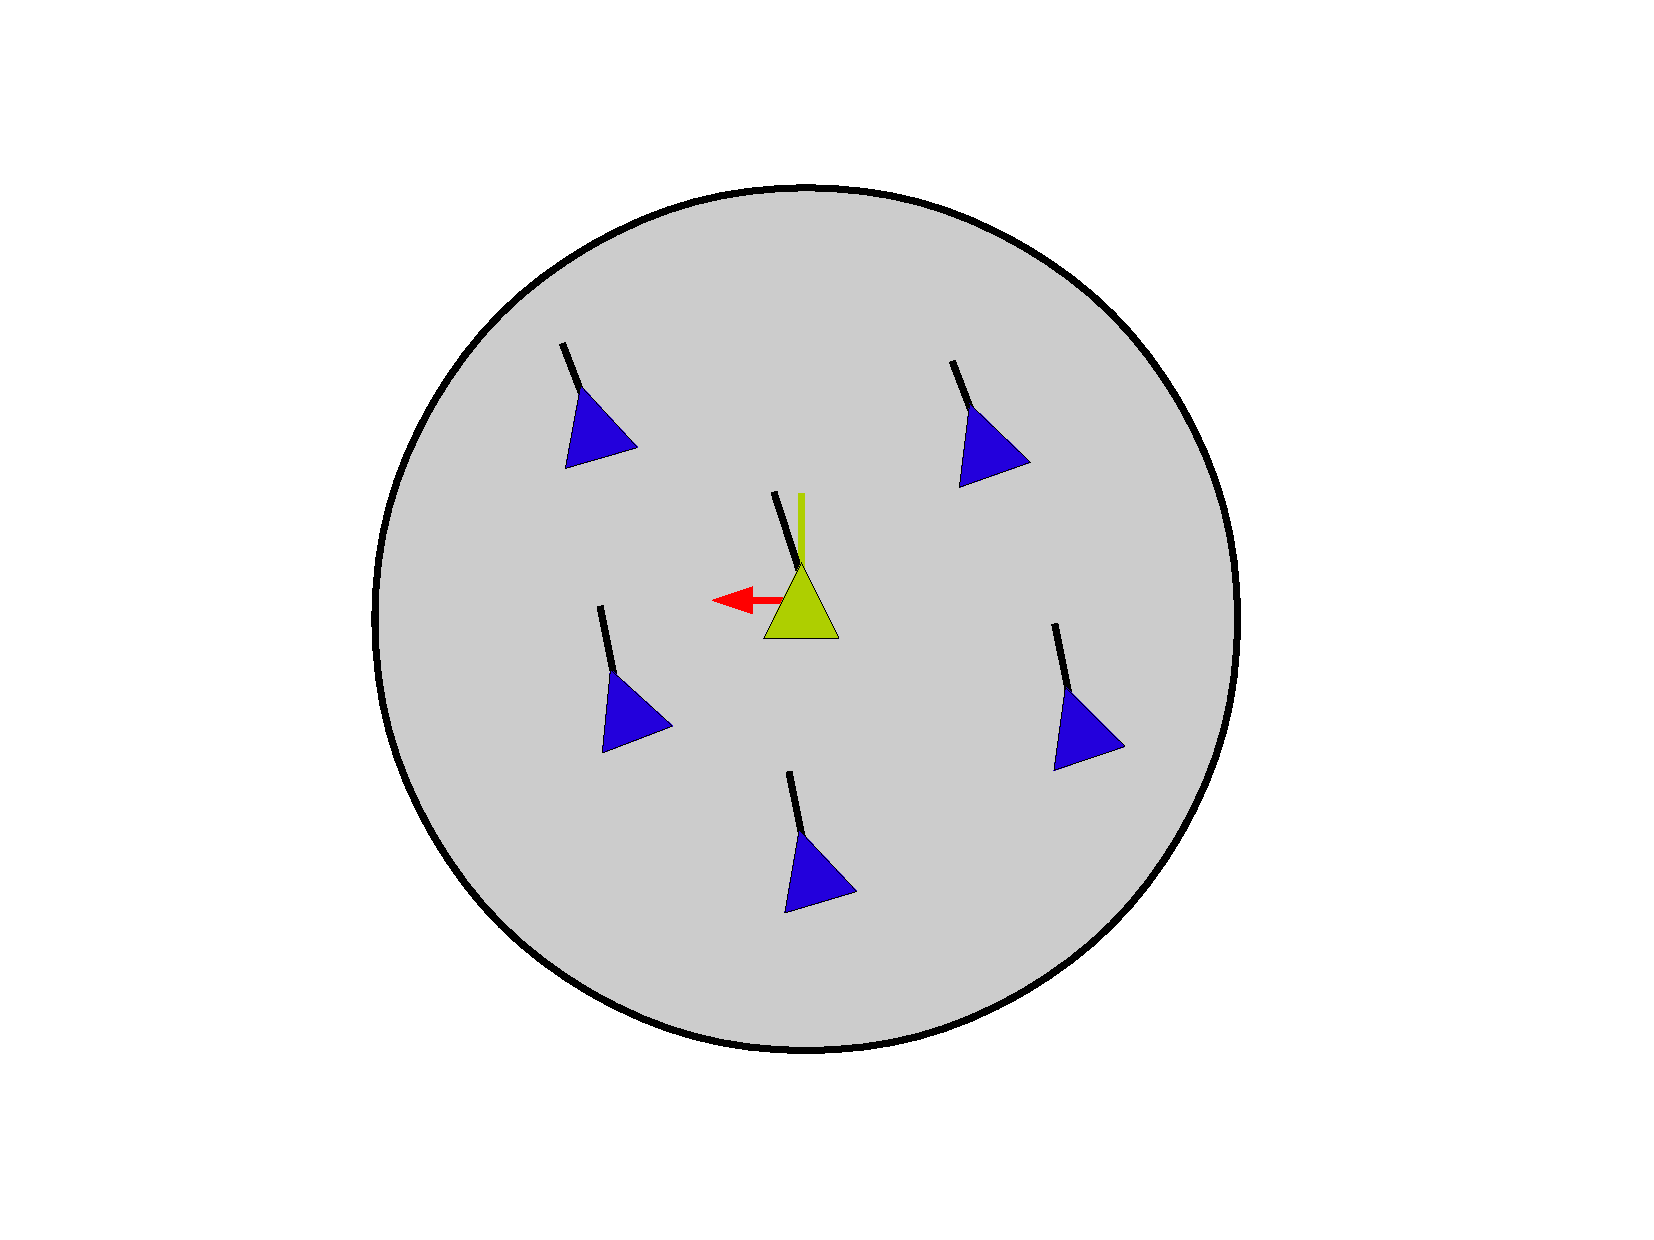
\includegraphics[scale=0.3]{figures/alignment.pdf}
\caption{Alignment steering force: the gray circle is the neighborhood of the green boid, \textit{alignment} match the heading and speed of the green boid with respect to the neighbors}
\label{alignmentPDF}
\end{center}
\end{figure}

\textit{Alignment} is also calculated in the local neighborhood of the boid in question. This steering behavior was computed using equation~\ref{alignmentEquation}.

% alignment equation
\begin{equation}
\label{alignmentEquation}
Alignment = \left[  \frac{1}{N} \sum_{n=1}^{N} v_n \right ] - v_i
\end{equation}

Where $N$ is the number of boids in the nearest neighbor within the search radius, this radius is bigger than the radius of the minimum separation distance used for \textit{separation}. $v_n$ is the velocity of boid $n$, average the velocities of all boids inside the neighbor, then subtract the velocity of the current boid from it to finally get the \textit{alignment} corrective force.

% cohesion
\subsection{Cohesion}
\textit{Cohesion} is the behavior that steers towards the center of the flock. When Reynolds introduced its \textit{Boids} model, he called this behavior \textit{flock centering} and defined it as \textit{the attempt to stay close to nearby objects}. The definition was kept while the name of the rule changed to \textit{cohesion}. This behavior makes each boid attracted to the center of the flock, in our case the calculation is using the local neighbor of each boid, so they would be attracted to the center of their local neighbor.  Figure~\ref{cohesionPDF} shows the \textit{cohesion} steering force in red.

% cohesion figure
\begin{figure}[htbp]
\begin{center}
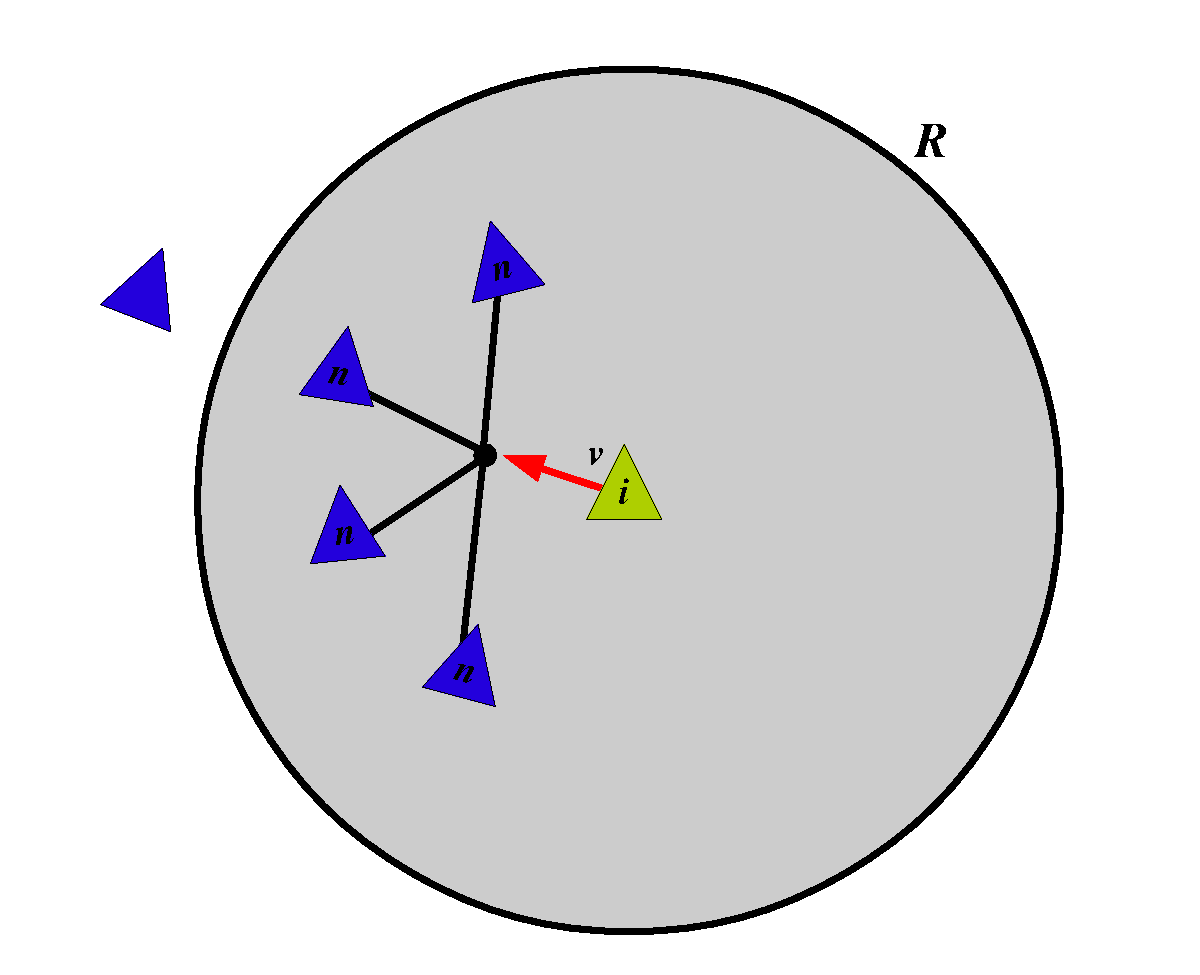
\includegraphics[scale=0.3]{figures/cohesion.pdf}
\caption{Cohesion steering force: the gray circle is the neighborhood of the green boid, \textit{cohesion} steers the green boid towards the center of their local neighborhood}
\label{cohesionPDF}
\end{center}
\end{figure}

The formula used for \textit{cohesion} is very similar to the formula used for \textit{alignment}, the only difference is that \textit{cohesion} uses the positions of the boid and \textit{alignment} uses the velocities. Equation~\ref{cohesionEquation} shows the \textit{cohesion} formula.

% cohesion equation
\begin{equation}
\label{cohesionEquation}
Cohesion = \left[  \frac{1}{N} \sum_{n=1}^{N} p_n \right ] - p_i
\end{equation}

Where $N$ is the number of boids in the local neighborhood of boid $i$. $p_n$ is the position of flockmate $n$. Then, take the average the position of the local flockmates in order to get the average position of the local neighborhood of boid $i$. Finally, subtract the current boid $i$ from the average position. That would give us the \textit{cohesion} force vector.

% other behaviors
\section{Other Steering Behaviors}\label{otherbehaviors}
Besides the three main steering behaviors discussed in the above section many more steering forces have been previously developed, see Section~\ref{currentwork} for a list of some of them. In this section only the behaviors that were implemented: \textit{goal}, \textit{avoid}, and \textit{follow the leader} are discussed.

% goal
\subsection{Goal}
\textit{Goal} is the steering behavior that attracts the boids to a specific location in global space. This location is static. Figure~\ref{seekfleePDF} shows the action taken when approaching or avoiding the target. The red vector shows the \textit{goal} steering, the blue vector, avoid, which is discussed in the next section. The gray vector to the right of the boid is the desired velocity and the dotted line would be the path taken by the boid.

% seek and flee figure
\begin{figure}[htbp]
\begin{center}
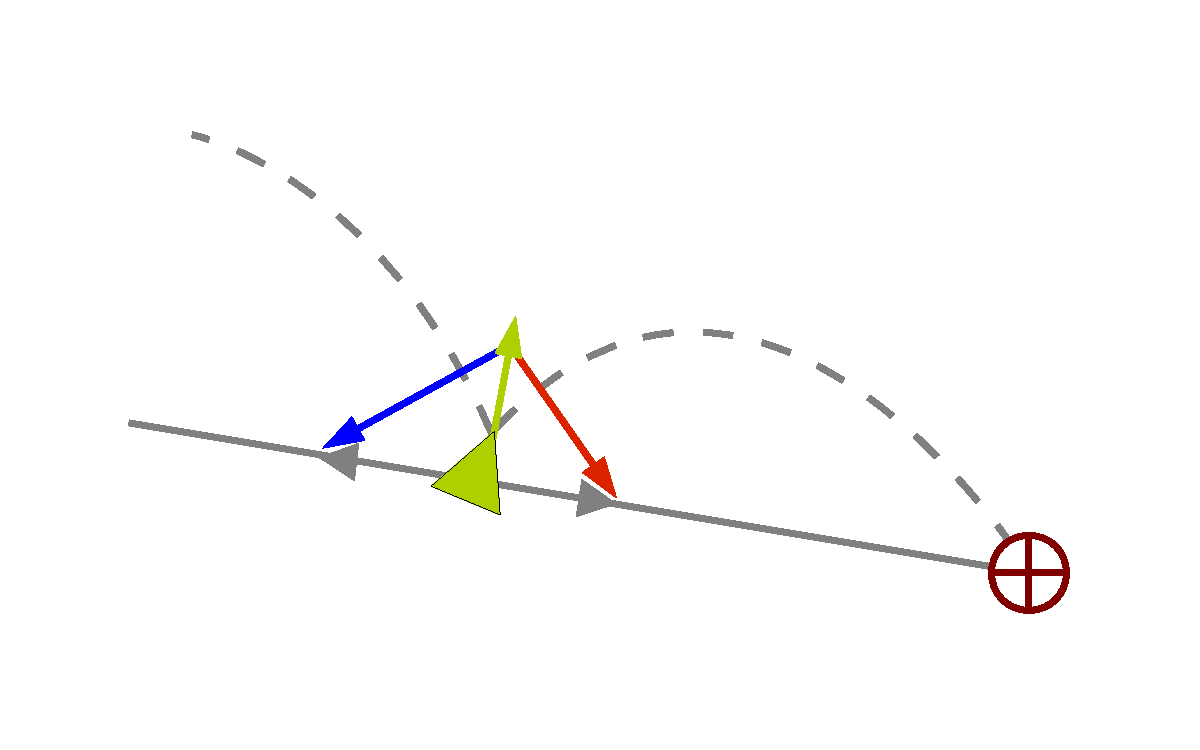
\includegraphics[scale=0.5]{figures/seekANDflee.pdf}
\caption{Goal and Avoid behaviors: the green boid would approach the target when is following the \textit{goal} behavior, or it would \textit{avoid} the target by backing out from it}
\label{seekfleePDF}
\end{center}
\end{figure}

\textit{Goal} behavior adjusts the boid's velocity in a way that it is aligned towards the target. So, \textit{how it was computed?} Since the target is static, subtract the position of the boid and the position of the target, normalize it and multiply it by the current speed of the boid. This gives us the desired velocity at which the boid is going to steer. Then, to get the steering vector, subtract the current velocity from the desired velocity. The formula is in equation~\ref{goalEquation}

% goal equation
\begin{equation}
\label{goalEquation}
Goal = ((p_i - p_t) * v_i) - v_i
\end{equation}

Where $p_i$ and $v_i$ are the position and velocity of boid $i$, respectively. This rule causes the boid to keep approaching the goal over and over, kind of like moth buzzing around a light bulb.

% avoid
\subsection{Avoid}
\textit{Avoid} means to steer away from a static target in the global space. The approach is similar to the one taken for \textit{goal} with the difference that the desired velocity will be pointing to the opposite direction. Figure~\ref{seekfleePDF} depicts the steering vector in blue and the desired velocity in gray (at the left side of the boid). Notice that the desire velocity vector for both \textit{goal} and \textit{avoid} are pointing in opposite directions. Equation~\ref{avoidEquation} shows the mathematical formula for \textit{avoid}.

% avoid equation
\begin{equation}
\label{avoidEquation}
Avoid = -((p_i - p_t) * v_i) - v_i
\end{equation}

$((p_i - p_t) * v_i)$ is called the desired velocity, and here it has a negative sign preceding it, so that means that it is going to point in the opposite direction than the desired velocity of ~\textit{goal}.

% leader following
\subsection{Follow the Leader}
\textit{Follow the Leader} is the behavior in which there is a boid in charge of the flock, called \textit{leader}, and the boids that follow it are the \textit{followers}. This is one of the many complex behaviors that a flock can exhibit. There is a pattern, individual boids evaluate different rules. Followers act like a point slightly behind the leader is its target, while the leader approaches randomly selected locations as its target.

% leader following figure
\begin{figure}[htbp]
\begin{center}
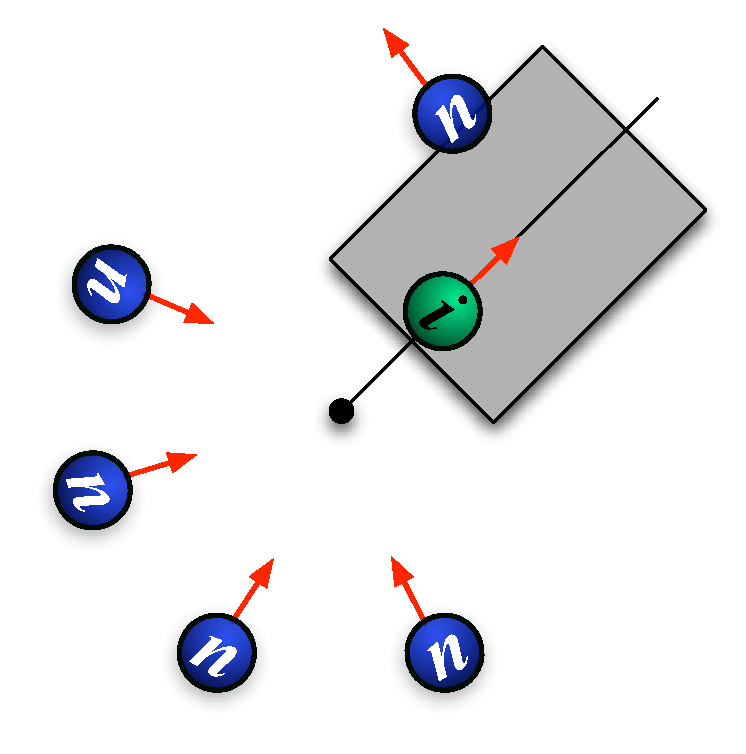
\includegraphics[scale=0.5]{figures/leaderFollowing.pdf}
\caption{Leader Following behavior: the followers would follow the leader by approaching a point slightly behind the leader, if a follower find itself in a rectangular area in front of the leader it would move out of the way of the leader}
\label{leaderPDF}
\end{center}
\end{figure}

Most of the time the followers want to stay closer to the leader without getting in its way. As can be seen in Figure~\ref{leaderPDF}.  If the follower is inside the rectangular region in front of the leader it moves away from it, leaving the way for the leader to move free without worrying about colliding with flockmates. The leader computes its movement using equation~\ref{goalEquation} where $p_t$ is a random position within the global space. The followers that are outside the rectangular region will approach a point slightly behind from the leader using equation~\ref{goalEquation}.

% combining behaviors
\section{Combining the Steering Behaviors}
Each of the steering behaviors discussed above would return a velocity vector. Now the question is \textit{how to combine the behaviors in order to move the boid?}. First, each steering force is normalized, then weight it\footnote{Weights are given by the user, they are not constant values set it by us.}. For example, combining \textit{separation}, \textit{alignment}, and \textit{cohesion} only, would be done using equation~\ref{combine}. Each behavior is multiplied by a constant, then add it to get the acceleration vector.

% combine equation
\begin{equation}
\label{combine}
acceleration = C_S Separation  + C_A Alignment  + C_C Cohesion 
\end{equation}

Now that the acceleration has been calculated, the velocity is just the acceleration plus the current velocity. See Equation~\ref{velocity}, where $v_i^{k+1}$ represents the velocity of boid $i$ at step $k+1$. 

Then, first order Euler integration method is used  to calculate the new position of each boid. As shown in Equation~\ref{integrate}, where $p_i^{k+1}$ is the position of boid $i$ at step $k+1$, $v_i$ is the velocity of the boid, and $dt$ is the time step of the integration.

% integrate equation
\begin{align}
\label{velocity}
v_i^{k+1} = v_i^k + acceleration\\
\label{integrate}
p_i^{k=1} = p_i^k + dt~ v_i
\end{align}

Each of the steering behaviors is going to be calculated, and combined for each boid every time step in order to update their positions.

% algorithm
\section{Algorithm}

In this Section a few algorithms are going to be presented. The first one is the algorithm developed to update all the boids at each frame of the simulation. The rest of them are the approaches taken to compute each of the steering behaviors that were implemented in the code to follow flocking behavior, this algorithms are executed at each time step.


% update
\begin{algorithm}
\caption{Update of each frame of the simulation}
\label{updateAlgorithm}
\begin{algorithmic}
\STATE Create a FLOCK particle system.
\FOR {each frame}
\STATE Do the nearest neighbor search.
\STATE Check if the weight of each rule is greater than zero, if it is then compute that rule.
\STATE Integrate over time.
\ENDFOR
\end{algorithmic}
\end{algorithm}

The Algorithm~\ref{updateAlgorithm} is a simplify version of what the \texttt{updateGPU()} function is doing. See Section~\ref{flocksection} for more details of the \texttt{updateGPU()} function. What is cleaver in this algorithm is that each of the rules is computed independently, not all at once. Only is the user set the weight greater than zero, then that rule is going to be computed. If the weight is zero, there is no waste of computation since the vector that stores the steering value for rule is initialized at zero and when combined, there is no error in the computation of the final steering.

Now internally, \textit{how the rules are computed?}. The following algorithms would present the approaches taken for each of the rules. Recalling that not all rules are going to be computed at once, only rules with weights greater than zero would be computed.


% flockmates
\begin{algorithm}
\caption{Compute the number of flockmates and nearest flockmates in the neighborhood.}
\label{flockmatesAlgorithm}
\begin{algorithmic}
\FOR {each neighbor $j$ of boid $i$}
\IF{dist($i$, $j$) $<=$ searching radius}
\STATE flockmates++
\IF{dist($i$, $j$) $<=$ minimum distance}
\STATE nearestFlockmates++
\ENDIF
\ENDIF
\ENDFOR
\end{algorithmic}
\end{algorithm}

Algorithm~\ref{flockmatesAlgorithm} counts how many flockmates and nearest flockmates are in the neighborhood of each boid. The number of flockmates is needed for the rules \textit{cohesion} and \textit{alignment} while the number of nearest flockmates is only needed by the \textit{separation} rule. The algorithm for the \textit{separation} rule is shown in Algorithm~\ref{separationAlgorithm}. In the \textit{separation} rule, only boids within the minimum distance are used for calculations. 

Algorithm~\ref{alignmentAlgorithm} presents how the \textit{alignment} rule is computed. This algorithm is very similar to the algorithm followed to computed \textit{cohesion}, shown in Algorithm~\ref{cohesionAlgorithm}. The only difference is that \textit{alignment} uses velocities while \textit{cohesion} uses positions.

% separation
\begin{algorithm}
\caption{Compute the separation steering behavior.}
\label{separationAlgorithm}
\begin{algorithmic}
\FOR {each neighbor $j$ of boid $i$}
\IF{dist($i$, $j$) $<=$ minimum distance}
\STATE s = $pos_i$ - $pos_j$ 
\STATE s /= dist($i$, $j$) 
\STATE separation += s
\ENDIF
\ENDFOR
\IF{nearestFlockmates $> 0$)}
\STATE separation /= nearestFlockmates
\ENDIF
\end{algorithmic}
\end{algorithm}




% alignment
\begin{algorithm}
\caption{Compute the alignment steering behavior.}
\label{alignmentAlgorithm}
\begin{algorithmic}
\FOR {each neighbor $j$ of boid $i$}
\IF{dist($i$, $j$) $<=$ searching radius}
\STATE alignment += velocity($j$)
\ENDIF
\ENDFOR
\IF{flockmates $> 0$)}
\STATE alignment /=  flockmates
\ENDIF
\STATE alignment -= velocity($i$)
\end{algorithmic}
\end{algorithm}

% cohesion
\begin{algorithm}
\caption{Compute the cohesion steering behavior.}
\label{cohesionAlgorithm}
\begin{algorithmic}
\FOR {each neighbor $j$ of boid $i$}
\IF{dist($i$, $j$) $<=$ searching radius}
\STATE cohesion += position($j$)
\ENDIF
\ENDFOR
\IF{flockmates $> 0$)}
\STATE cohesiont /=  flockmates
\ENDIF
\STATE cohesion -= position($i$)
\end{algorithmic}
\end{algorithm}
